\documentclass{beamer}
\usepackage[utf8]{inputenc}
\usepackage[T1]{fontenc}
\usepackage[english,italian]{babel}
\usepackage{amsmath}
\usepackage{amssymb}
\usepackage{amsfonts}
\usepackage{mathrsfs}
\usepackage{graphicx}
\usepackage{amsthm}
\usepackage{newlfont}
\usepackage{color}
\usepackage{natbib}
\usepackage{float}
\usepackage{textcomp}
\usetheme{Frankfurt}
\usecolortheme{beaver}
%\usetheme{CambridgeUS}

\setbeamertemplate{caption}{\raggedright\insertcaption\par}


\begin{document}
\title{\textcolor{black}{Analisi della complessità di reti neurali generate tramite algoritmi genetici}}
\author{Mattia Ceccarelli}
\date{18 ottobre 2018}
\institute{Università di Bologna}

\begin{frame}
 \maketitle
\end{frame}

\begin{frame}
 \frametitle{Introduzione}
 \begin{enumerate}
 \item[-]Algoritmi Genetici
 \begin{enumerate}
 \item[-]
 \end{enumerate}
 \item[-]Reti Neurali
 \end{enumerate}

\end{frame}

\begin{frame}
 \frametitle{Algoritmi Genetici}

\end{frame}
\begin{frame}
 \frametitle{Reti Neurali}
\end{frame}

\begin{frame}
 \frametitle{Dataset}
 \begin{figure}
  \centering
  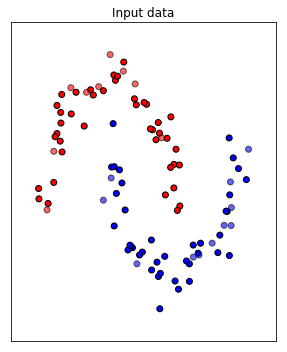
\includegraphics[scale = 0.5]{images/moons_noise.png}
  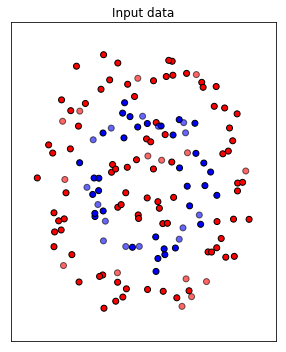
\includegraphics[scale = 0.5]{images/circles+_noise.png}
  \caption{\large A sinistra \textit{Moons} e a destra \textit{Circles+} con noise = 0.2}
 \end{figure}

\end{frame}

\begin{frame}
 \frametitle{Classificazione su \textit{Moons}}
 \begin{figure}[H]
 \centering
 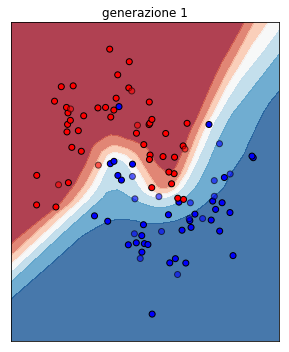
\includegraphics[scale = 0.25]{images/moons-rnd-log./1.png}
 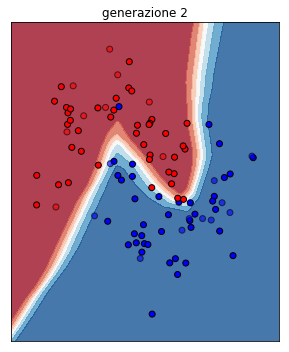
\includegraphics[scale = 0.25]{images/moons-rnd-log./2.png}
 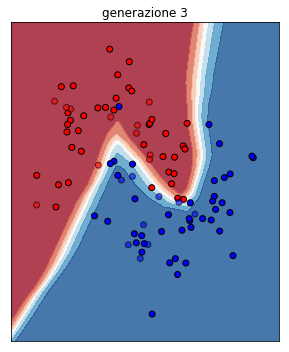
\includegraphics[scale = 0.25]{images/moons-rnd-log./3.png}
 \\
 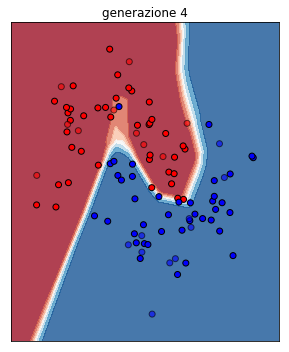
\includegraphics[scale = 0.25]{images/moons-rnd-log./4.png}
 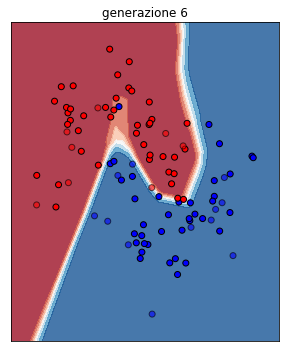
\includegraphics[scale = 0.25]{images/moons-rnd-log./5.png}
 \caption{\large Esempio di evoluzione nella classificazione di \textit{Moons}}
 \end{figure}
\end{frame}

\begin{frame}
 \frametitle{Classificazione su \textit{Circles+}}
 \begin{figure}
  \centering
  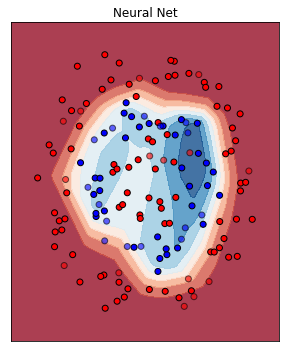
\includegraphics[scale = 0.25]{images/circle+-rnd-log./1.png}
  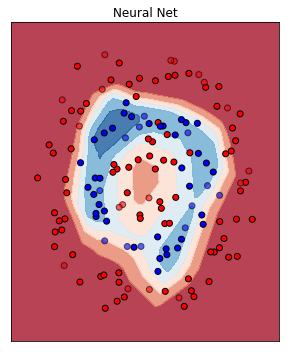
\includegraphics[scale = 0.25]{images/circle+-rnd-log./2.png}
  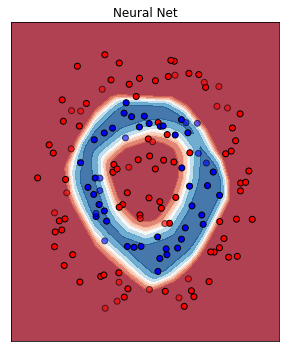
\includegraphics[scale = 0.25]{images/circle+-rnd-log./3.png}
  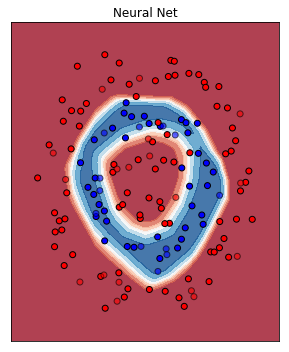
\includegraphics[scale = 0.25]{images/circle+-rnd-log./4.png}
  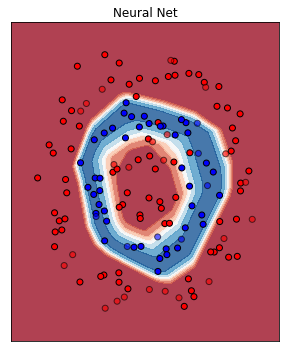
\includegraphics[scale = 0.25]{images/circle+-rnd-log./5.png}
  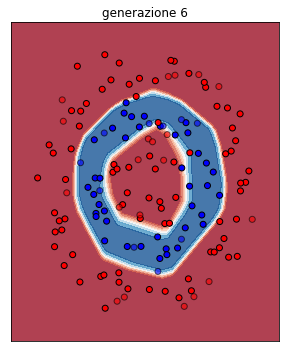
\includegraphics[scale = 0.25]{images/circle+-rnd-log./6.png}
  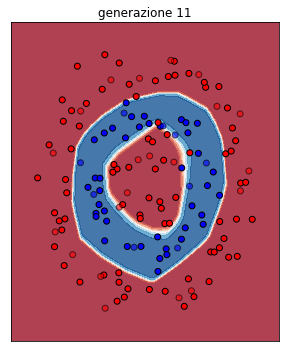
\includegraphics[scale = 0.25]{images/circle+-rnd-log./11.png}
  \caption{\large Esempio di evoluzione nella classificazione di \textit{Circles+}}
 \end{figure}   
\end{frame}

\begin{frame}
 \frametitle{Analisi della complessità}
 La rumorosità dei dataset modifica alcuni parametri della rete:
 \begin{enumerate}
  \item [-] Score
  \item [-] Numero di collegamenti (Links)
  \item [-] Lunghezza (o profondità) ossia il numero di hidden layer 
  \item [-] Numero di neuroni nel layer più piccolo
 \end{enumerate}
 Gli ultimi tre sono quelli che quantificano la complessità della rete 
\end{frame}

\begin{frame}
 \frametitle{Score su \textit{Moons} e \textit{Circles+}}
  \begin{figure}[H]
   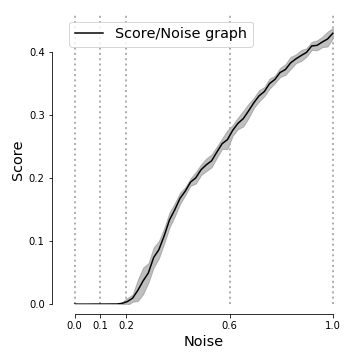
\includegraphics[scale = 0.42]{images/score_noise_moons.png}
   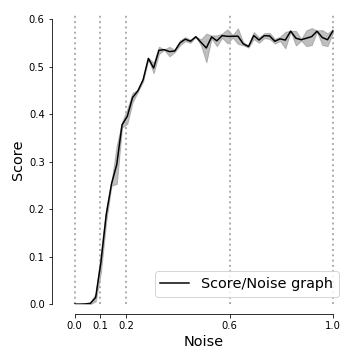
\includegraphics[scale = 0.42]{images/score_noise_circles+.png}
   \caption{\large Andamento dello score in funzione del noise in \textit{Moons} (a sinistra) e sul dataset \textit{circles+} (a destra)}
    \end{figure}

\end{frame}

\begin{frame}
 \frametitle{Links su \textit{Moons} e \textit{Circles+}}
 \begin{figure}
 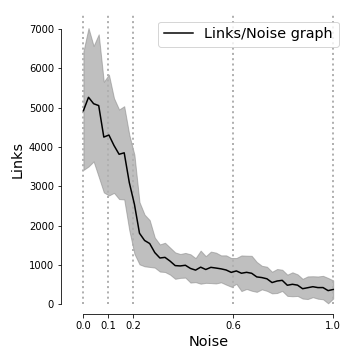
\includegraphics[scale = 0.42]{images/links_noise_moons.png}
 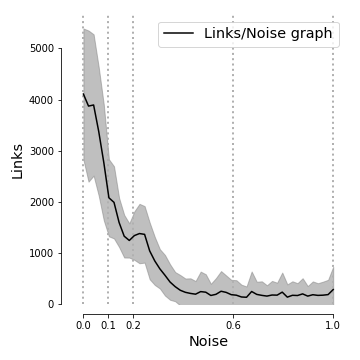
\includegraphics[scale = 0.42]{images/links_noise_circles+.png}
 \caption{\large Numero di collegamenti in funzione del noise su \textit{Moons} (a sinistra) e \textit{Circles+} (a destra)}
 \end{figure}
\end{frame}

\begin{frame}
 \frametitle{Layer più piccolo della rete }
    \begin{figure}
    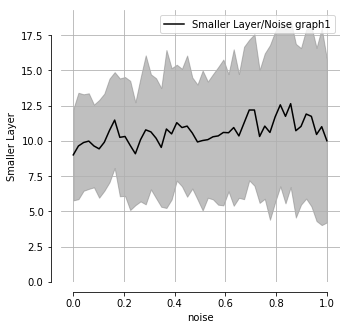
\includegraphics[scale = 0.42]{images/small_noise_moons.png}
    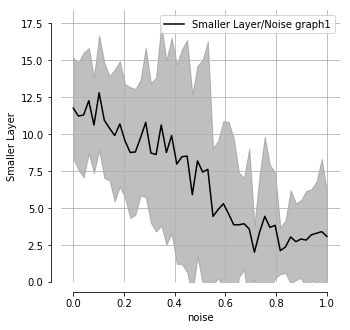
\includegraphics[scale = 0.42]{images/small_noise_circles+.png}
    \caption{\large Numero di neuroni nel layer più piccolo della rete su \textit{Moons} (a sinistra) e su \textit{Circles+} (a destra)}
 \end{figure}
\end{frame}

\begin{frame}
 \frametitle{Lunghezza}
 \begin{figure}
 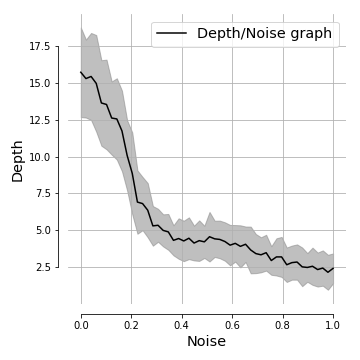
\includegraphics[scale = 0.42]{images/depth_noise_moons.png}
 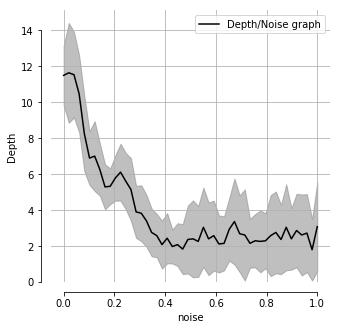
\includegraphics[scale = 0.42]{images/depth_noise_circles+.png}
 \caption{\large Numero di Hidden Layer della rete in funzione del noise su \textit{Moons} (a sinistra) e \textit{Circles+} (a destra)}
 
 \end{figure}
\end{frame}

\begin{frame}
 \frametitle{Conclusioni}
\end{frame}

\begin{frame}
 \frametitle{Sviluppi Futuri}
\end{frame}




\end{document}
